% !Mode:: "TeX:UTF-8"
% Author: Rickjin (ZhihuiJin@gmail.com)
%
\chapter{LDA 数学八卦}
\section{开篇}

在 Machine Learning 中,LDA 是两个常用模型的简称: Linear Discriminant Analysis 和 Latent Dirichlet Allocation,
在这篇文章中我们主要八卦的是后者。LDA 是一个在文本建模中很著名的模型,类似于 SVD, PLSA 等模型, 可以用于浅层语义分析,在文本语义分析中是一个很有用的模型。很不幸的是,这个模型中涉及的数学知识有点多,
包括 Gamma 函数, Dirichlet 分布, Dirichlet-Multinomial 共轭, Gibbs Sampling,
Variational Inference, 贝叶斯文本建模,PLSA 建模, 以及 LDA 文本建模。

这篇文章的主要目标,就是科普在学习理解LDA 模型中,需要了解的一些重要的数学知识。
预设的读者是做自然语言处理、机器学习、数据挖掘方向的工程师,
要读懂这篇科普,需要的数学基础知识基本上不超过陈希孺先生的《概率论与数理统计》这本书。

文章标题挂上“八卦”两字, 因为八卦意味着自由、不拘束、可以天马行空,细节处理上也难免有不严谨的地方;
当然我也希望八卦是相对容易理解的,即便他是关于数学的八卦。对于本文中的任何评论,
欢迎发信到我的新浪微博帐号 rickjin, 或者是邮箱 zhihuijin@gmail.com。


\section{文本建模}

我们日常生活中总是产生大量的文本,如果每一个文本存储为一篇文档,那
每篇文档从人的观察来说就是有序的词的序列 $d=(w_1, w_2, \cdots, w_n)$。

\begin{figure}[htbp]
\centering
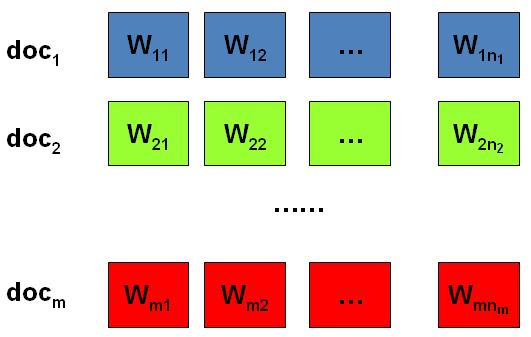
\includegraphics[width=0.5\textwidth]{lda/corpus.jpg}
\caption{包含$m$ 篇文档的语料库}
\end{figure}

统计文本建模的目的就是追问这些观察到语料库中的的词序列是如何生成的。
统计学被人们描述为猜测上帝的游戏,人类产生的所有的语料文本我们都可以看成是一个伟大的上帝在
天堂中抛掷骰子生成的,我们观察到的只是上帝玩这个游戏的结果 ------ 词序列构成的语料,
而上帝玩这个游戏的过程对我们是个黑盒子。所以在统计文本建模中,我们希望猜测出上帝是如何玩这个游戏的,
具体一点,最核心的两个问题是
\begin{enumerate}
\item 上帝都有什么样的骰子;
\item 上帝是如何抛掷这些骰子的;
\end{enumerate}

第一个问题就是表示模型中都有哪些参数,骰子的每一个面的概率都对应于模型中的参数;
第二个问题就表示游戏规则是什么,上帝可能有各种不同类型的骰子,
上帝可以按照一定的规则抛掷这些骰子从而产生词序列。

\begin{figure}[htbp]
\centering
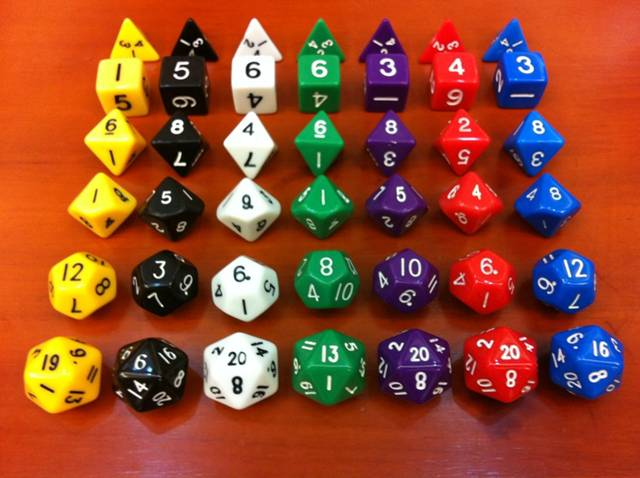
\includegraphics[width=0.41\textwidth]{lda/dice-all.jpg} \quad
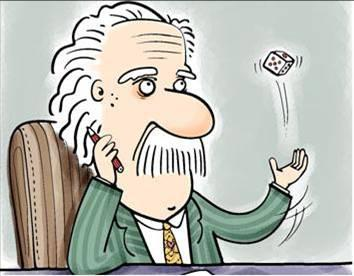
\includegraphics[width=0.4\textwidth]{lda/god-throw-dice.jpg}
\caption{上帝掷骰子}
\end{figure}

\subsection{Unigram Model}
假设我们的词典中一共有 $V$ 个词 $v_1, v_2, \cdots v_V$,那么最简单的 Unigram Model 就是
认为上帝是按照如下的游戏规则产生文本的。

\begin{algorithm}[!ht]
\floatname{algorithm}{Game}
\caption{Unigram Model}
\begin{algorithmic}[1]
\STATE 上帝只有一个骰子,这个骰子有 $V$ 个面, 每个面对应一个词, 各个面的概率不一;
\STATE 每抛一次骰子,抛出的面就对应的产生一个词;如果一篇文档中有 $n$ 个词,上帝就是独立的抛$n$次骰子产生这$n$ 个词;
\end{algorithmic}
\end{algorithm}

上帝的这个唯一的骰子各个面的概率记为 $\vec{p} = (p_1, p_2, \cdots, p_V)$,
所以每次投掷骰子类似于一个抛钢镚时候的贝努利实验, 
只是贝努利实验中我们抛的是一个两面的骰子,而此处抛的是一个$V$面的骰子,
我们把抛这个$V$面骰子的实验记为记为 $w\sim Mult(w|\vec{p}) $。
\begin{figure}[htbp]
\centering
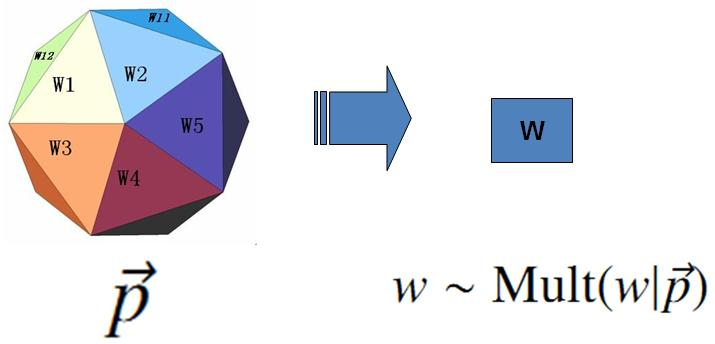
\includegraphics[width=0.4\textwidth]{lda/unigram-model.jpg}
\caption{上帝投掷$V$ 个面的骰子}
\end{figure}

对于一篇文档$d=\vec{w}=(w_1, w_2, \cdots, w_n)$, 该文档被生成的概率就是
$$ p(\vec{w}) = p(w_1, w_2, \cdots, w_n) = p(w_1)p(w_2) \cdots p(w_n) $$
而文档和文档之间我们认为是独立的, 所以如果语料中有多篇文档
$\mathcal{W}=(\vec{w_1}, \vec{w_2},...,\vec{w_m})$,
则该语料的概率是
$$p(\mathcal{W})= p(\vec{w_1})p(\vec{w_2})
\cdots p(\vec{w_m}) $$

在 Unigram Model 中, 我们假设了文档之间是独立可交换的,而文档中的词也是独立可交换的,
所以一篇文档相当于一个袋子,里面装了一些词,而词的顺序信息就无关紧要了,
这样的模型也称为词袋模型(Bag-of-words)。

假设语料中总的词频是$N$, 在所有的 $N$ 个词中,如果我们关注每个词 $v_i$ 的发生次数 $n_i$,
那么 $\vec{n}=(n_1, n_2,\cdots, n_V)$ 正好是一个多项分布
$$ p(\vec{n}) = Mult(\vec{n}|\vec{p}, N)
= \binom{N}{\vec{n}} \prod_{k=1}^V p_k^{n_k} $$
此时, 语料的概率是
\begin{align*}
p(\mathcal{W})= p(\vec{w_1})p(\vec{w_2}) \cdots p(\vec{w_m})
= \prod_{k=1}^V p_k^{n_k}
\end{align*}

当然,我们很重要的一个任务就是估计模型中的参数$\vec{p}$,
也就是问上帝拥有的这个骰子的各个面的概率是多大,按照统计学家中频率派的观点,使
用最大似然估计最大化$P(\mathcal{W})$,于是参数$p_i$的估计值就是
$$ \hat{p_i} = \frac{n_i}{N} .$$

对于以上模型,贝叶斯统计学派的统计学家会有不同意见,
他们会很挑剔的批评只假设上帝拥有唯一一个固定的骰子是不合理的。
在贝叶斯学派看来,一切参数都是随机变量,以上模型中的骰子 $\vec{p}$不是唯一固定的,
它也是一个随机变量。所以按照贝叶斯学派的观点,上帝是按照以下的过程在玩游戏的
\begin{algorithm}[H]
\floatname{algorithm}{Game}
\caption{贝叶斯 Unigram Model假设}
\begin{algorithmic}[1]
\STATE 上帝有一个装有无穷多个骰子的坛子,里面有各式各样的骰子,每个骰子有 $V$ 个面;
\STATE 上帝从坛子里面抽了一个骰子出来,然后用这个骰子不断的抛,然后产生了语料中的所有的词;
\end{algorithmic}
\end{algorithm}
上帝的这个坛子里面,骰子可以是无穷多个,有些类型的骰子数量多,有些类型的骰子少,所以从概率分布的角度看,
坛子里面的骰子$\vec{p}$ 服从一个概率分布 $p(\vec{p})$,这个分布称为参数
$\vec{p}$ 的先验分布。

\begin{figure}[htbp]
\centering
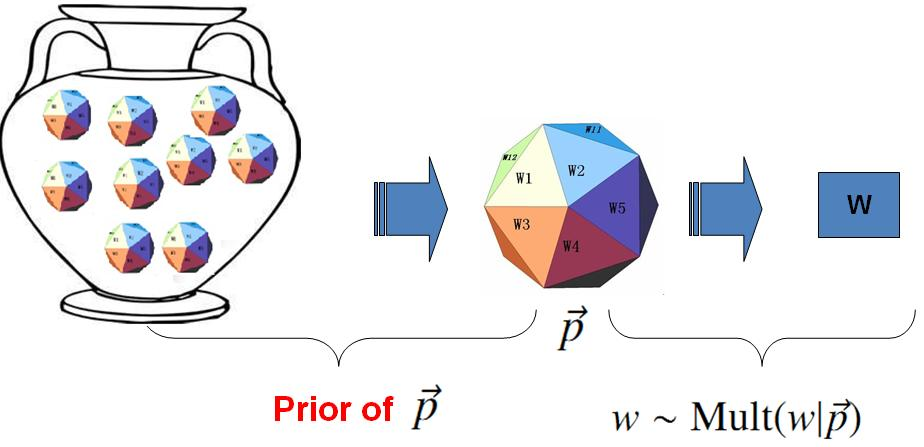
\includegraphics[width=0.6\textwidth]{lda/bayesian-unigram-model.jpg}
\caption{贝叶斯观点下的 Unigram Model}
\end{figure}

以上贝叶斯学派的游戏规则的假设之下,语料$\mathcal{W}$产生的概率如何计算呢?
由于我们并不知道上帝到底用了哪个骰子$\vec{p}$,所以每个骰子都是可能被使用的,
只是使用的概率由先验分布$p(\vec{p})$来决定。
对每一个具体的骰子$\vec{p}$,由该骰子产生数据的概率是 $p(\mathcal{W}|\vec{p})$,
所以最终数据产生的概率就是对每一个骰子$\vec{p}$上产生的数据概率进行积分累加求和
$$ p(\mathcal{W}) = \int p(\mathcal{W}|\vec{p}) p(\vec{p})d\vec{p} $$
在贝叶斯分析的框架下,此处先验分布$p(\vec{p})$ 就可以有很多种选择了,注意到
$$ p(\vec{n}) = Mult(\vec{n}|\vec{p}, N) $$ 实际上是在计算一个多项分布的概率,所以对先验分布的一个比较好的选择就是多项分布对应的共轭分布,
即 Dirichlet 分布
$$ Dir(\vec{p}|\vec{\alpha})=
\frac{1}{\Delta(\vec{\alpha})} \prod_{k=1}^V p_k^{\alpha_k -1},
\quad \vec{\alpha}=(\alpha_1, \cdots, \alpha_V) $$
此处,$\Delta(\vec{\alpha})$ 就是归一化因子$Dir(\vec{\alpha})$,即
$$ \Delta(\vec{\alpha}) =
\int \prod_{k=1}^V p_k^{\alpha_k -1} d\vec{p} . $$

\begin{figure}[htbp]
\centering
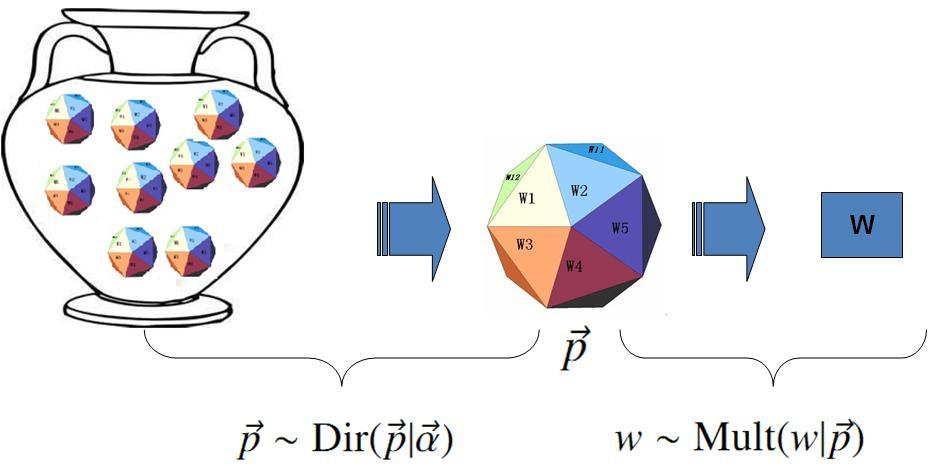
\includegraphics[width=0.5\textwidth]{lda/dirichlet-multinomial-unigram.jpg}
\caption{Dirichlet 先验下的 Unigram Model}
\end{figure}
\begin{figure}[htbp]
\centering
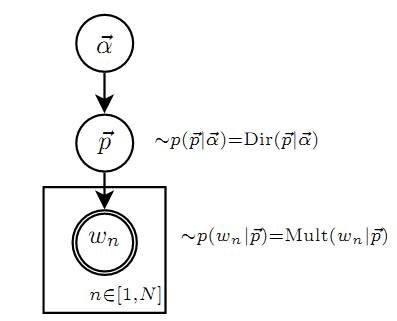
\includegraphics[width=0.4\textwidth]{lda/graph-model-unigram.jpg}
\caption{Unigram Model的概率图模型}
\end{figure}

回顾前一个小节介绍的 Drichlet 分布的一些知识,其中很重要的一点就是
\begin{center}
\bf{Dirichlet 先验 + 多项分布的数据
$\longrightarrow$ 后验分布为 Dirichlet 分布}
$$ Dir(\vec{p}|\vec{\alpha}) + MultCount(\vec{n})
 = Dir(\vec{p}|\vec{\alpha}+\vec{n}) $$
\end{center}
于是,在给定了参数 $\vec{p}$的先验分布 $Dir(\vec{p}|\vec{\alpha})$ 的时候,
各个词出现频次的数据 $\vec{n} \sim Mult(\vec{n}|\vec{p},N)$ 为多项分布,
所以无需计算,我们就可以推出后验分布是
\begin{equation}
p(\vec{p}|\mathcal{W},\vec{\alpha})
= Dir(\vec{p}|\vec{n}+ \vec{\alpha})
= \frac{1}{\Delta(\vec{n}+\vec{\alpha})}
\prod_{k=1}^V p_k^{n_k + \alpha_k -1}
\end{equation}

在贝叶斯的框架下,参数$\vec{p}$如何估计呢?由于我们已经有了参数的后验分布,
所以合理的方式是使用后验分布的极大值点,或者是参数在后验分布下的平均值。
在该文档中,我们取平均值作为参数的估计值。使用上个小节中\eqref{dir-mean}式的结论,
由于 $\vec{p}$ 的后验分布为 $Dir(\vec{p}|\vec{n} + \vec{\alpha})$,于是
$$
 E(\vec{p}) = \Bigl(\frac{n_1 + \alpha_1}{\sum_{i=1}^V(n_i + \alpha_i)},
 \frac{n_2 + \alpha_2}{\sum_{i=1}^V(n_i + \alpha_i)}, \cdots,
 \frac{n_V + \alpha_V}{\sum_{i=1}^V(n_i + \alpha_i)} \Bigr)
$$
也就是说对每一个 $p_i$, 我们用下式做参数估计
\begin{equation}
\label{dirichlet-parameter-estimation}
 \hat{p_i} = \frac{n_i + \alpha_i}{\sum_{i=1}^V(n_i + \alpha_i)}
\end{equation}
考虑到 $\alpha_i$ 在 Dirichlet 分布中的物理意义是事件的先验的伪计数,这个估计式子的含义是很直观的:
每个参数的估计值是其对应事件的先验的伪计数和数据中的计数的和在整体计数中的比例。

进一步,我们可以计算出文本语料的产生概率为
\begin{align}
p(\mathcal{W}|\vec{\alpha}) & = \int p(\mathcal{W}|\vec{p}) p(\vec{p}|\vec{\alpha})d\vec{p} \notag  \\
& = \int \prod_{k=1}^V p_k^{n_k} Dir(\vec{p}|\vec{\alpha}) d\vec{p} \notag  \\
& = \int \prod_{k=1}^V p_k^{n_k} \frac{1}{\Delta(\vec{\alpha})}
\prod_{k=1}^V p_k^{\alpha_k -1} d\vec{p} \notag  \\
& = \frac{1}{\Delta(\vec{\alpha})}
\int \prod_{k=1}^V p_k^{n_k + \alpha_k -1} d\vec{p} \notag \\
& = \frac{\Delta(\vec{n}+\vec{\alpha})}{\Delta(\vec{\alpha})}
\label{likelihood-dir-mult}
\end{align}

\subsection{Topic Model 和 PLSA}
以上 Unigram Model 是一个很简单的模型,模型中的假设看起来过于简单,
和人类写文章产生每一个词的过程差距比较大,有没有更好的模型呢?

我们可以看看日常生活中人是如何构思文章的。如果我们要写一篇文章,往往是先确定要写哪几个主题。
譬如构思一篇自然语言处理相关的文章,可能 40\% 会谈论语言学、30\% 谈论概率统计、20\% 谈论计算机、
还有10\%谈论其它的主题:
\begin{itemize}
\item 说到语言学,我们容易想到的词包括:语法、句子、乔姆斯基、句法分析、主语...;
\item 谈论概率统计,我们容易想到以下一些词: 概率、模型、均值、方差、证明、独立、马尔科夫链、...;
\item 谈论计算机,我们容易想到的词是: 内存、硬盘、编程、二进制、对象、算法、复杂度...;
\end{itemize}
我们之所以能马上想到这些词,是因为这些词在对应的主题下出现的概率很高。
我们可以很自然的看到,一篇文章通常是由多个主题构成的、
而每一个主题大概可以用与该主题相关的频率最高的一些词来描述。

以上这种直观的想法由Hoffmn 于 1999 年给出的PLSA(Probabilistic Latent Semantic Analysis) 模型中
首先进行了明确的数学化。Hoffman 认为一篇文档(Document) 可以由多个主题(Topic) 混合而成, 而每个Topic 都是词汇上的概率分布,文章中的每个词都是由一个固定的 Topic 生成的。下图是英语中几个Topic 的例子。
\begin{figure}[htbp]
\centering
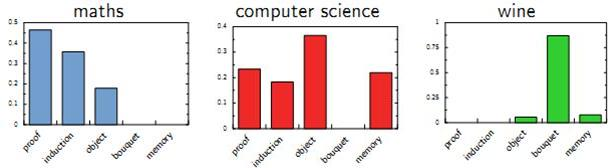
\includegraphics[width=1.0\textwidth]{lda/topic-examples.jpg}
\caption{Topic 就是Vocab 上的概率分布}
\end{figure}

所有人类思考和写文章的行为都可以认为是上帝的行为,我们继续回到上帝的假设中,那么在 PLSA 模型中,Hoffman 认为上帝是按照如下的游戏规则来生成文本的。
\begin{algorithm}[htb]
\floatname{algorithm}{Game}
\caption{PLSA Topic Model }
\begin{algorithmic}[1]
\STATE 上帝有两种类型的骰子,一类是 doc-topic 骰子,每个 doc-topic 骰子有 $K$ 个面,每个面是一个 topic 的编号;
一类是 topic-word 骰子,每个 topic-word 骰子有 $V$ 个面, 每个面对应一个词;
\begin{center}
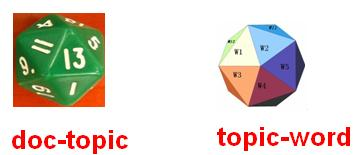
\includegraphics[width=0.4\textwidth]{lda/topic-model-dice.jpg}
\end{center}

\STATE 上帝一共有 $K$ 个 topic-word 骰子, 每个骰子有一个编号,编号从 $1$ 到$K$;
\STATE 生成每篇文档之前,上帝都先为这篇文章制造一个特定的 doc-topic 骰子,
然后重复如下过程生成文档中的词
\begin{itemize}
\item 投掷这个 doc-topic 骰子,得到一个 topic 编号 $z$
\item 选择 $K$ 个 topic-word 骰子中编号为$z$的那个,投掷这个骰子,于是得到一个词
\end{itemize}
\end{algorithmic}
\end{algorithm}

以上PLSA 模型的文档生成的过程可以图形化的表示为
\begin{figure}[H]
\centering
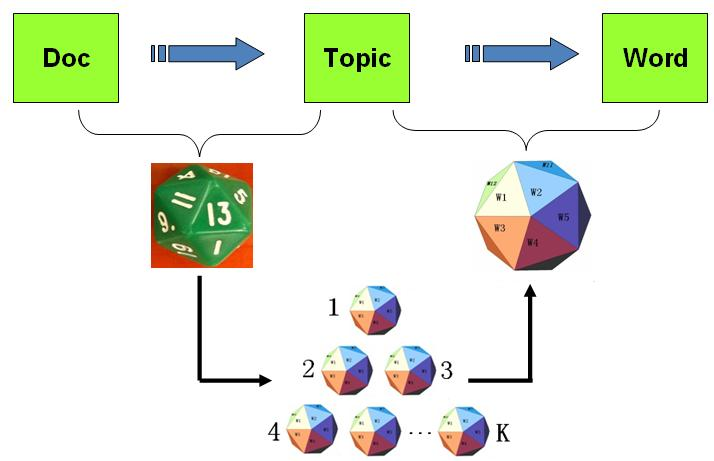
\includegraphics[width=0.6\textwidth]{lda/plsa-doc-topic-word.jpg}
\caption{PLSA 模型的文档生成过程}
\end{figure}

我们可以发现在以上的游戏规则下,文档和文档之间是独立可交换的,
同一个文档内的词也是独立可交换的,还是一个 bag-of-words 模型。
游戏中的$K$ 个topic-word 骰子,我们可以记为 $\vec{\varphi}_1, \cdots, \vec{\varphi}_K$,
对于包含$M$篇文档的语料 $C=(d_1, d_2, \cdots, d_M)$ 中的每篇文档$d_m$,
都会有一个特定的doc-topic骰子$\vec{\theta}_m$,
所有对应的骰子记为 $\vec{\theta}_1, \cdots, \vec{\theta}_M$。
为了方便,我们假设每个词$w$ 都是一个编号,对应到topic-word 骰子的面。
于是在 PLSA 这个模型中,第$m$篇文档 $d_m$ 中的每个词的生成概率为
$$ p(w|d_m) = \sum_{z=1}^K p(w|z)p(z|d_m) = \sum_{z=1}^K \varphi_{zw} \theta_{mz}$$
所以整篇文档的生成概率为
$$ p(\vec{w}|d_m) = \prod_{i=1}^n \sum_{z=1}^K p(w_i|z)p(z|d_m) =
\prod_{i=1}^n \sum_{z=1}^K \varphi_{zw_i} \theta_{dz} $$
由于文档之间相互独立,我们也容易写出整个语料的生成概率。
求解PLSA 这个 Topic Model 的过程汇总,模型参数并容易求解,
可以使用著名的 EM 算法进行求得局部最优解,
由于该模型的求解并不是本文的介绍要点,
有兴趣的同学参考 Hoffman 的原始论文,此处略去不讲。

\section{LDA 文本建模}

\subsection{游戏规则}
对于上述的 PLSA 模型,贝叶斯学派显然是有意见的,doc-topic 骰子$\vec{\theta}_m$
和 topic-word 骰子$\vec{\varphi}_k$都是模型中的参数,参数都是随机变量,怎么能没有先验分布呢?
于是,类似于对 Unigram Model 的贝叶斯改造, 我们也可以如下在两个骰子参数前加上先验分布从而
把 PLSA 对应的游戏过程改造为一个贝叶斯的游戏过程。
由于 $\vec{\varphi}_k$和$\vec{\theta}_m$都对应到多项分布,
所以先验分布的一个好的选择就是Drichlet 分布,
于是我们就得到了 LDA(Latent Dirichlet Allocation)模型。
\begin{figure}[htbp]
\centering
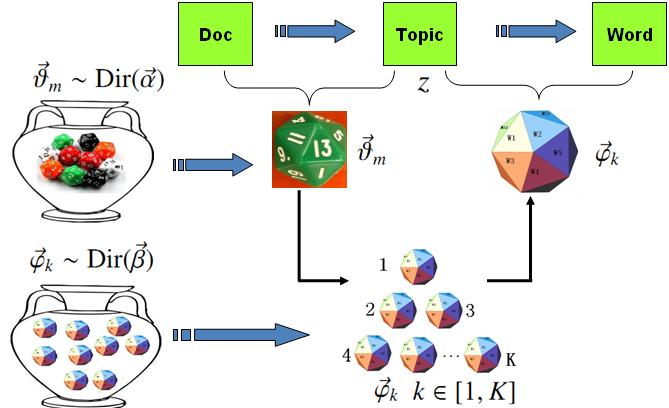
\includegraphics[width=0.8\textwidth]{lda/lda-dice.jpg}
\caption{LDA模型}
\end{figure}

在 LDA 模型中, 上帝是按照如下的规则玩文档生成的游戏的
\begin{algorithm}[H]
\floatname{algorithm}{Game}
\caption{LDA Topic Model }
\begin{algorithmic}[1]
\STATE 上帝有两大坛子的骰子,第一个坛子装的是 doc-topic 骰子,第二个坛子装的是 topic-word 骰子;
\begin{center}
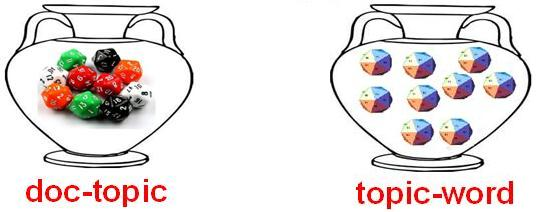
\includegraphics[width=0.4\textwidth]{lda/lda-dice-urn.jpg}
\end{center}

\STATE 上帝随机的从第二个坛子中独立的抽取了 $K$ 个 topic-word 骰子,编号为 $1$ 到$K$;
\STATE 每次生成一篇新的文档前,上帝先从第一个坛子中随机抽取一个 doc-topic 骰子,然后重复如下过程生成文档中的词
\begin{itemize}
\item 投掷这个 doc-topic 骰子,得到一个 topic 编号 $z$
\item 选择 $K$ 个 topic-word 骰子中编号为$z$的那个,投掷这个骰子,于是得到一个词
\end{itemize}
\end{algorithmic}
\end{algorithm}

假设语料库中有 $M$ 篇文档,所有的的word和对应的 topic 如下表示
\begin{align*}
\vec{\mathbf{w}} & = (\vec{w}_1, \cdots, \vec{w}_M) \\
\vec{\mathbf{z}} & = (\vec{z}_1, \cdots, \vec{z}_M)
\end{align*}
其中, $\vec{w}_m$ 表示第$m$ 篇文档中的词, $\vec{z}_m$ 表示这些词对应的 topic 编号。
\begin{figure}[H]
\centering
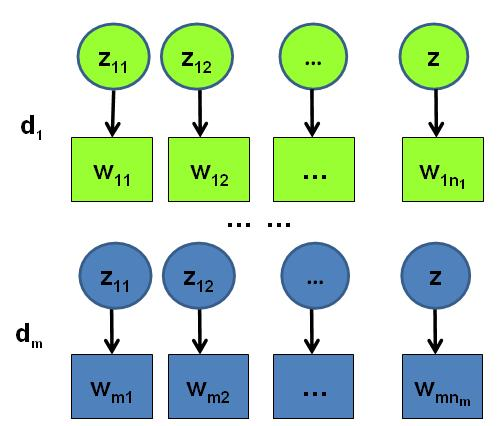
\includegraphics[width=0.5\textwidth]{lda/word-topic-vector.jpg}
\caption{语料生成过程中的 word 和 topic}
\end{figure}

\subsection{物理过程分解}
使用概率图模型表示, LDA 模型的游戏过程如图所示。
\begin{figure}[H]
\centering
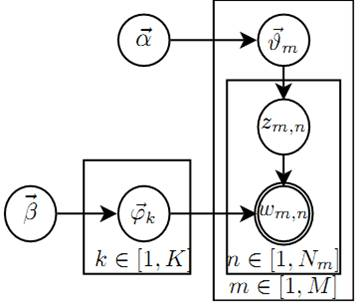
\includegraphics[width=0.4\textwidth]{lda/lda-graph-model.jpg}
\caption{LDA图模型表示}
\end{figure}


这个概率图可以分解为两个主要的物理过程:
\begin{enumerate}
\item $\vec{\alpha}\rightarrow \vec{\theta}_m \rightarrow  z_{m,n}$, 这个过程
表示在生成第$m$ 篇文档的时候,先从第一个坛子中抽了一个doc-topic 骰子 $\vec{\theta}_m$,
然后投掷这个骰子生成了文档中第 $n$ 个词的topic编号$z_{m,n}$;

\item $\vec{\beta} \rightarrow \vec{\varphi}_k \rightarrow w_{m,n} | k=z_{m,n}$,
这个过程表示用如下动作生成语料中第$m$篇文档的第 $n$个词:
在上帝手头的$K$ 个topic-word 骰子 $\vec{\varphi}_k$ 中,
挑选编号为 $k=z_{m,n}$的那个骰子进行投掷,
然后生成 word $w_{m,n}$;
\end{enumerate}

理解 LDA最重要的就是理解这两个物理过程。 LDA 模型在基于 $K$ 个 topic
生成语料中的 $M$ 篇文档的过程中, 由于是 bag-of-words 模型,有一些物理过程是相互独立可交换的。
由此, LDA 生成模型中, $M$ 篇文档会对应于 $M$ 个独立的 Dirichlet-Multinomial 共轭结构;
$K$ 个 topic 会对应于 $K$ 个独立的 Dirichlet-Multinomial 共轭结构。所以理解 LDA 所需要的所有数学
就是理解 Dirichlet-Multiomail 共轭,其它都就是理解物理过程。
现在我们进入细节, 来看看 LDA 模型是如何被分解为 $M+K$ 个Dirichlet-Multinomial 共轭结构的。


由第一个物理过程,我们知道
$\vec{\alpha}\rightarrow \vec{\theta}_m \rightarrow  \vec{z}_{m}$
表示生成第 $m$ 篇文档中的所有词对应的topics,
显然  $\vec{\alpha}\rightarrow \vec{\theta}_m $ 对应于 Dirichlet 分布,
$\vec{\theta}_m \rightarrow  \vec{z}_{m}$ 对应于 Multinomial 分布, 所以整体是一个
Dirichlet-Multinomial 共轭结构;
$$ \vec{\alpha}\underbrace{\xrightarrow{\hspace*{2cm}}}_{Dirichlet} \vec{\theta}_m
\underbrace{\xrightarrow{\hspace*{2cm}}}_{Multinomial} \vec{z}_{m} $$
前文介绍 Bayesian Unigram Model 的小节中我们对 Dirichlet-Multinomial 共轭结构做了一些计算。
借助于该小节中的\eqref{likelihood-dir-mult}式,我们可以得到
$$ p(\vec{z}_m |\vec{\alpha}) = \frac{\Delta(\vec{n}_m+\vec{\alpha})}{\Delta(\vec{\alpha})} $$
其中 $\vec{n}_m = (n_{m}^{(1)}, \cdots, n_{m}^{(K)})$,
$n_{m}^{(k)}$ 表示第$m$篇文档中第$k$ 个topic 产生的词的个数。
进一步,利用 Dirichlet-Multiomial 共轭结构,我们得到参数 $\vec{\theta}_m$ 的后验分布恰好是
$$Dir(\vec{\theta}_m| \vec{n}_m + \vec{\alpha}).$$

由于语料中 $M$篇文档的 topics 生成过程相互独立,所以我们得到 $M$ 个相互独立的
Dirichlet-Multinomial 共轭结构,从而我们可以得到整个语料中 topics 生成概率
\begin{align}
\label{corpus-topic-prob}
p(\vec{\mathbf{z}} |\vec{\alpha}) & = \prod_{m=1}^M p(\vec{z}_m |\vec{\alpha}) \notag \\
&= \prod_{m=1}^M \frac{\Delta(\vec{n}_m+\vec{\alpha})}{\Delta(\vec{\alpha})}
\end{align}

目前为止,我们由$M$篇文档得到了 $M$ 个 Dirichlet-Multinomial 共轭结构,
还有额外$K$ 个 Dirichlet-Multinomial 共轭结构在哪儿呢?
在上帝按照之前的规则玩 LDA 游戏的时候,上帝是先完全处理完成一篇文档,再处理下一篇文档。
文档中每个词的生成都要抛两次骰子,第一次抛一个doc-topic骰子得到 topic,
第二次抛一个topic-word骰子得到 word,每次生成每篇文档中的一个词的时候这两次抛骰子的动作是紧邻轮换进行的。
如果语料中一共有 $N$ 个词,则上帝一共要抛 $2N$次骰子,轮换的抛doc-topic骰子和 topic-word骰子。
但实际上有一些抛骰子的顺序是可以交换的,我们可以等价的调整$2N$次抛骰子的次序:
前$N$次只抛doc-topic骰子得到语料中所有词的 topics,然后基于得到的每个词的 topic 编号,
后$N$次只抛topic-word骰子生成 $N$ 个word。于是上帝在玩 LDA 游戏的时候,
可以等价的按照如下过程进行:

\begin{algorithm}[H]
\floatname{algorithm}{Game}
\caption{LDA Topic Model 2}
\begin{algorithmic}[1]
\STATE 上帝有两大坛子的骰子,第一个坛子装的是 doc-topic 骰子,第二个坛子装的是 topic-word 骰子;
\STATE 上帝随机的从第二个坛子中独立的抽取了 $K$ 个 topic-word 骰子,编号从 $1$ 到$K$;
\STATE 每次生成一篇新的文档前,上帝先从第一个坛子中随机抽取一个 doc-topic 骰子,
然后重复投掷这个 doc-topic 骰子,为每个词生成一个 topic 编号 $z$;
重复如上过程处理每篇文档,生成语料中每个词的 topic 编号,但是词尚未生成;
\STATE 从头到尾,对语料中的每篇文档中的每个 topic 编号 $z$, 选择 $K$ 个 topic-word 骰子中编号为$z$的那个,投掷这个骰子,于是生成对应的word;
\end{algorithmic}
\end{algorithm}

以上游戏是先生成了语料中所有词的 topic, 然后对每个词在给定 topic 的条件下生成 word。
在语料中所有词的 topic 已经生成的条件下,任何两个 word 的生成动作都是可交换的。
于是我们把语料中的词进行交换,把具有相同 topic 的词放在一起
\begin{align*}
\vec{\mathbf{w}}' &= (\vec{w}_{(1)}, \cdots, \vec{w}_{(K)}) \\
\vec{\mathbf{z}}' &= (\vec{z}_{(1)}, \cdots, \vec{z}_{(K)})
\end{align*}
其中,$\vec{w}_{(k)}$ 表示这些词都是由第 $k$ 个 topic 生成的,
$\vec{z}_{(k)}$ 对应于这些词的 topic 编号,所以$\vec{z}_{(k)}$中的分量都是$k$。

对应于概率图中的第二个物理过程
$\vec{\beta} \rightarrow \vec{\varphi}_k \rightarrow w_{m,n} | k=z_{m,n}$,
在 $k=z_{m,n}$ 的限制下,语料中任何两个由 topic $k$ 生成的词
都是可交换的,即便他们不再同一个文档中,所以我们此处不再考虑文档的概念,
转而考虑由同一个 topic 生成的词。考虑如下过程
$\vec{\beta} \rightarrow \vec{\varphi}_k \rightarrow \vec{w}_{(k)}$ ,
容易看出, 此时 $\vec{\beta} \rightarrow \vec{\varphi}_k $ 对应于 Dirichlet 分布,
$ \vec{\varphi}_k \rightarrow \vec{w}_{(k)}$ 对应于 Multinomial 分布, 所以整体也还是一个
Dirichlet-Multinomial 共轭结构;

$$ \vec{\beta}\underbrace{\xrightarrow{\hspace*{2cm}}}_{Dirichlet} \vec{\varphi}_k
\underbrace{\xrightarrow{\hspace*{2cm}}}_{Multinomial} \vec{w}_{(k)} $$
同样的借助于\eqref{likelihood-dir-mult}式,我们可以得到
$$ p(\vec{w}_{(k)} |\vec{\beta}) = \frac{\Delta(\vec{n}_k+\vec{\beta})}{\Delta(\vec{\beta})} $$
其中 $\vec{n}_k = (n_{k}^{(1)}, \cdots, n_{k}^{(V)})$,
$n_{k}^{(t)}$ 表示第$k$ 个topic 产生的词中 word $t$的个数。
进一步,利用 Dirichlet-Multiomial 共轭结构,我们得到参数 $ \vec{\varphi}_k$ 的后验分布恰好是
$$Dir( \vec{\varphi}_k| \vec{n}_k + \vec{\beta}).$$


而语料中 $K$个 topics 生成words 的过程相互独立,所以我们得到 $K$ 个相互独立的
Dirichlet-Multinomial 共轭结构,从而我们可以得到整个语料中词生成概率
\begin{align}
\label{corpus-word-prob}
p(\vec{\mathbf{w}} |\vec{\mathbf{z}},\vec{\beta}) &= p(\vec{\mathbf{w}}' |\vec{\mathbf{z}}',\vec{\beta}) \notag \\
&= \prod_{k=1}^K p(\vec{w}_{(k)} | \vec{z}_{(k)}, \vec{\beta}) \notag \\
&= \prod_{k=1}^K \frac{\Delta(\vec{n}_k+\vec{\beta})}{\Delta(\vec{\beta})}
\end{align}

结合 \eqref{corpus-topic-prob} 和 \eqref{corpus-word-prob} 于是我们得到
\begin{align}
\label{lda-corpus-likelihood}
p(\vec{\mathbf{w}},\vec{\mathbf{z}} |\vec{\alpha}, \vec{\beta}) &=
p(\vec{\mathbf{w}} |\vec{\mathbf{z}}, \vec{\beta}) p(\vec{\mathbf{z}} |\vec{\alpha})  \notag \\
&= \prod_{k=1}^K \frac{\Delta(\vec{n}_k+\vec{\beta})}{\Delta(\vec{\beta})}
\prod_{m=1}^M \frac{\Delta(\vec{n}_m+\vec{\alpha})}{\Delta(\vec{\alpha})}
\end{align}

此处的符号表示稍微不够严谨, 向量 $\vec{n}_k$,  $\vec{n}_m$ 都用 $n$ 表示, 主要通过下标进行区分,
$k$ 下标为 topic 编号, $m$ 下标为文档编号。

\subsection{Gibbs Sampling}
有了联合分布 $p(\vec{\mathbf{w}},\vec{\mathbf{z}})$, 万能的 MCMC 算法就可以发挥作用了!
于是我们可以考虑使用 Gibbs Sampling 算法对这个分布进行采样。
当然由于 $\vec{\mathbf{w}}$ 是观测到的已知数据,只有 $\vec{\mathbf{z}}$是隐含的变量,
所以我们真正需要采样的是分布 $p(\vec{\mathbf{z}}|\vec{\mathbf{w}})$。在 Gregor Heinrich
那篇很有名的LDA 模型科普文章 \emph{Parameter estimation for text analysis} 中,是基于
\eqref{lda-corpus-likelihood} 式推导 Gibbs Sampling 公式的。此小节中我们使用不同的方式,主要是基于
Dirichlet-Multinomial 共轭来推导 Gibbs Sampling 公式,这样对于理解采样中的概率物理过程有帮助。

语料库$\vec{\mathbf{z}}$ 中的第$i$个词对应的 topic 我们记为$z_i$, 其中$i=(m,n)$是一个二维下标,
对应于第$m$篇文档的第 $n$个词,我们用 $\neg i$ 表示去除下标为$i$的词。那么按照 Gibbs Sampling 算法的要求,
我们要求得任一个坐标轴 $i$ 对应的条件分布 $p(z_i = k|\vec{\mathbf{z}}_{\neg i}, \vec{\mathbf{w}})$ 。
假设已经观测到的词 $w_i = t$, 则由贝叶斯法则,我们容易得到
\begin{align*}
p(z_i = k|\vec{\mathbf{z}}_{\neg i}, \vec{\mathbf{w}}) \propto
p(z_i = k, w_i = t |\vec{\mathbf{z}}_{\neg i}, \vec{\mathbf{w}}_{\neg i}) \\
\end{align*}
由于$z_i = k, w_i = t$ 只涉及到第 $m$ 篇文档和第$k$个 topic,所以上式的条件概率计算中,
实际上也只会涉及到如下两个Dirichlet-Multinomial 共轭结构
\begin{enumerate}
\item $\vec{\alpha} \rightarrow \vec{\theta}_m \rightarrow  \vec{z}_{m}$
\item $\vec{\beta} \rightarrow \vec{\varphi}_k \rightarrow \vec{w}_{(k)}$
\end{enumerate}
其它的 $M+K-2$ 个 Dirichlet-Multinomial 共轭结构和$z_i = k, w_i = t$是独立的。

由于在语料去掉第$i$ 个词对应的 $(z_i, w_i)$,
并不改变我们之前讨论的 $M+K$ 个 Dirichlet-Multinomial 共轭结构,只是某些地方的计数会减少。
所以$\vec{\theta}_m, \vec{\varphi}_k$ 的后验分布都是 Dirichlet:
\begin{align*}
p(\vec{\theta}_m|\vec{\mathbf{z}}_{\neg i}, \vec{\mathbf{w}}_{\neg i})
&= Dir(\vec{\theta}_m| \vec{n}_{m,\neg i} + \vec{\alpha}) \\
p(\vec{\varphi}_k|\vec{\mathbf{z}}_{\neg i}, \vec{\mathbf{w}}_{\neg i})
&=  Dir( \vec{\varphi}_k| \vec{n}_{k,\neg i} + \vec{\beta})
\end{align*}
使用上面两个式子,把以上想法综合一下,我们就得到了如下的 Gibbs Sampling 公式的推导
\begin{align*}
p(z_i = k|\vec{\mathbf{z}}_{\neg i}, \vec{\mathbf{w}}) & \propto
p(z_i = k, w_i = t |\vec{\mathbf{z}}_{\neg i}, \vec{\mathbf{w}}_{\neg i}) \\
&= \int p(z_i = k, w_i = t, \vec{\theta}_m,\vec{\varphi}_k |
   \vec{\mathbf{z}}_{\neg i}, \vec{\mathbf{w}}_{\neg i}) d \vec{\theta}_m d \vec{\varphi}_k \\
&= \int p(z_i = k, \vec{\theta}_m|\vec{\mathbf{z}}_{\neg i}, \vec{\mathbf{w}}_{\neg i})
   \cdot p(w_i = t, \vec{\varphi}_k | \vec{\mathbf{z}}_{\neg i}, \vec{\mathbf{w}}_{\neg i})
   d \vec{\theta}_m d \vec{\varphi}_k   \\
&= \int p(z_i = k |\vec{\theta}_m) p(\vec{\theta}_m|\vec{\mathbf{z}}_{\neg i}, \vec{\mathbf{w}}_{\neg i})
   \cdot p(w_i = t |\vec{\varphi}_k) p(\vec{\varphi}_k|\vec{\mathbf{z}}_{\neg i}, \vec{\mathbf{w}}_{\neg i})
   d \vec{\theta}_m d \vec{\varphi}_k   \\
&= \int p(z_i = k |\vec{\theta}_m) Dir(\vec{\theta}_m| \vec{n}_{m,\neg i} + \vec{\alpha})  d \vec{\theta}_m \\
& \hspace{0.2cm} \cdot \int p(w_i = t |\vec{\varphi}_k) Dir( \vec{\varphi}_k| \vec{n}_{k,\neg i} + \vec{\beta}) d \vec{\varphi}_k \\
&= \int \theta_{mk} Dir(\vec{\theta}_m| \vec{n}_{m,\neg i} + \vec{\alpha})  d \vec{\theta}_m
    \cdot \int \varphi_{kt} Dir( \vec{\varphi}_k| \vec{n}_{k,\neg i} + \vec{\beta})  d \vec{\varphi}_k   \\
&= E(\theta_{mk}) \cdot E(\varphi_{kt}) \\
&= \hat{\theta}_{mk} \cdot \hat{\varphi}_{kt} \\
\label{gibbs-sampling-deduction}
\end{align*}

以上推导估计是整篇文章中最复杂的数学了,表面上看上去复杂,
但是推导过程中的概率物理意义是简单明了的:$z_i = k, w_i = t $的概率
只和两个 Dirichlet-Multinomail 共轭结构关联。而最终得到的 $\hat{\theta}_{mk}, \hat{\varphi}_{kt}$
就是对应的两个 Dirichlet 后验分布在贝叶斯框架下的参数估计。
借助于前面介绍的Dirichlet 参数估计的公式 \eqref{dirichlet-parameter-estimation},我们有
\begin{align*}
\hat{\theta}_{mk} &= \frac{n_{m,\neg i}^{(k)} + \alpha_k}{\sum_{k=1}^K (n_{m,\neg i}^{(t)} + \alpha_k)} \\
\hat{\varphi}_{kt} &= \frac{n_{k,\neg i}^{(t)} + \beta_t}{\sum_{t=1}^V (n_{k,\neg i}^{(t)} + \beta_t)}
\end{align*}
于是,我们最终得到了 LDA 模型的 Gibbs Sampling 公式
\begin{equation}
\label{gibbs-sampling}
p(z_i = k|\vec{\mathbf{z}}_{\neg i}, \vec{\mathbf{w}})  \propto
\frac{n_{m,\neg i}^{(k)} + \alpha_k}{\sum_{k=1}^K (n_{m,\neg i}^{(t)} + \alpha_k)}
\cdot \frac{n_{k,\neg i}^{(t)} + \beta_t}{\sum_{t=1}^V (n_{k,\neg i}^{(t)} + \beta_t)}
\end{equation}

这个公式是很漂亮的, 右边其实就是 $p(topic|doc) \cdot p(word|topic)$,这个概率其实是 $doc \rightarrow topic \rightarrow word$ 的路径概率,由于topic 有$K$ 个,所以 Gibbs Sampling 公式的物理意义其实就是在这$K$ 条路径中
进行采样。

\begin{figure}[H]
\centering
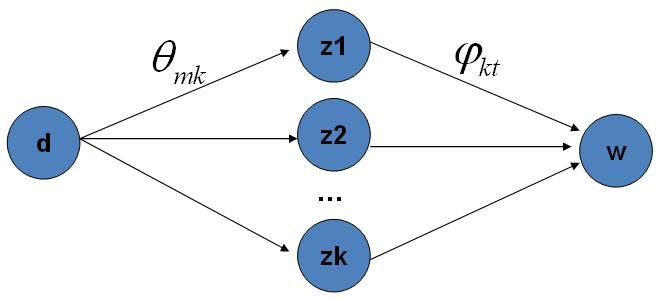
\includegraphics[width=0.6\textwidth]{lda/gibbs-path-search.jpg}
\caption{doc-topic-word 路径概率}
\end{figure}

\subsection{Training and Inference}

有了 LDA 模型,当然我们的目标有两个
\begin{itemize}
\item 估计模型中的参数 $\vec{\varphi}_1, \cdots, \vec{\varphi}_K$ 和 $\vec{\theta}_1, \cdots, \vec{\theta}_M$;
\item 对于新来的一篇文档$doc_{new}$,我们能够计算这篇文档的 topic 分布$\vec{\theta}_{new}$。
\end{itemize}

有了 Gibbs Sampling 公式, 我们就可以基于语料训练 LDA 模型,并应用训练得到的模型对新的文档进行
topic 语义分析。训练的过程就是通过Gibbs Sampling 获取语料中的 $(z,w)$ 的样本,
而模型中的所有的参数都可以基于最终采样得到的样本进行估计。
训练的流程很简单:
\begin{algorithm}[H]
\caption{LDA Training}
\begin{algorithmic}[1]
\STATE 随机初始化:对语料中每篇文档中的每个词$w$,随机的赋一个 topic 编号$z$;
\STATE 重新扫描语料库,对每个词$w$, 按照 Gibbs Sampling 公式重新采样它的 topic,在语料中进行更新;
\STATE 重复以上语料库的重新采样过程直到 Gibbs Sampling 收敛;
\STATE 统计语料库的 topic-word 共现频率矩阵,该矩阵就是 LDA的模型;
\end{algorithmic}
\end{algorithm}

对于 Gibbs Sampling 算法实现的细节,请参考 Gregor Heinrich 的 \emph{Parameter estimation for text analysis}
中对算法的描述,以及 \href{http://code.google.com/p/plda}{PLDA} 的代码实现,此处不再赘述。

由这个topic-word 频率矩阵我们可以计算每一个$p(word|topic)$概率,从而算出
模型参数$\vec{\varphi}_1, \cdots, \vec{\varphi}_K$, 这就是上帝用的 $K$ 个 topic-word 骰子。
当然,语料中的文档对应的骰子参数 $\vec{\theta}_1, \cdots, \vec{\theta}_M$ 在以上训练过程中
也是可以计算出来的,只要在 Gibbs Sampling 收敛之后,统计每篇文档中的 topic 的频率分布,我们就可以计算
每一个 $p(topic|doc)$ 概率,于是就可以计算出每一个$\vec{\theta}_m$。
由于参数$\vec{\theta}_m$ 是和训练语料中的每篇文档相关的,对于我们理解新的文档并无用处,所以
工程上最终存储 LDA 模型时候一般没有必要保留。通常,在 LDA 模型训练的过程中,
我们是取 Gibbs Sampling 收敛之后的 $n$ 个迭代的结果进行平均来做参数估计,这样模型质量更高。

有了 LDA 的模型,对于新来的文档 $doc_{new}$, 我们如何做该文档的 topic 语义分布的计算呢?
基本上 inference 的过程和 training 的过程完全类似。
对于新的文档, 我们只要认为 Gibbs Sampling 公式中的 $\hat{\varphi}_{kt}$ 部分是稳定不变的,
是由训练语料得到的模型提供的,所以采样过程中
我们只要估计该文档的 topic 分布$\vec{\theta}_{new}$就好了。

\begin{algorithm}[H]
\caption{LDA Inference}
\begin{algorithmic}[1]
\STATE 随机初始化:对当前文档中的每个词$w$,随机的赋一个 topic 编号$z$;
\STATE 重新扫描当前文档,按照 Gibbs Sampling 公式,对每个词$w$, 重新采样它的 topic;
\STATE 重复以上过程直到 Gibbs Sampling 收敛;
\STATE 统计文档中的topic分布,该分布就是 $\vec{\theta}_{new}$
\end{algorithmic}
\end{algorithm}


\section{后记}

LDA 对于专业做机器学习的兄弟而言,只能算是一个简单的Topic Model。
但是对于互联网中做数据挖掘、语义分析的工程师,LDA 的门槛并不低。
LDA 典型的属于这样一种机器学习模型:要想理解它,需要比较多的数学背景,要在工程上进行实现,却相对简单。
Gregor Heinrich 的LDA 模型科普文章 \emph{Parameter estimation for text analysis} 写得非常的出色,
这是学习 LDA 的必看文章。不过即便是这篇文章,对于工程师也是有门槛的。
我写的这个科普最好对照 Gregor Heinrich 的这篇文章来看, 我用的数学符号也是尽可能和这篇文章保持一致。

这份LDA 科普是基于给组内兄弟做报告的 ppt 整理而成的,说是科普其实也不简单,涉及到的数学
还是太多。在工业界也混了几年,经常感觉到工程师对于
学术界的玩的模型有很强的学习和尝试的欲望,只是学习成本往往太高。所以我写 LDA 的初衷就是写给工业界
的工程师们看的,希望把学术界玩的一些模型用相对通俗的方式介绍给工程师;如果这个科普对于读研究生的
一些兄弟姐妹也有所启发,只能说那是一个 side effect :-)。

我个人很喜欢LDA ,它是在文本建模中一个非常优雅的模型,相比于很多其它的贝叶斯模型,
LDA 在数学推导上简洁优美。学术界自 2003 年以来也输出了很多基于LDA 的 Topic Model 的变体,
要想理解这些更加高级的 Topic Model, 首先需要很好的理解标准的 LDA 模型。
在工业界, Topic Model 在 Google、Baidu
等大公司的产品的语义分析中都有着重要的应用;
所以Topic Model 对于工程师而言,这是一个很有应用价值、值得学习的模型。
我接触 Topic Model 的时间不长,主要是由于2年前和 PLDA 的作者 Wangyi 一起合作的过程中,
从他身上学到了很多 Topic Model 方面的知识。关于 LDA 的相关知识,其实可以写的还有很多:
如何提高 LDA Gibbs Sampling 的速度、如何优化超参数、如何做大规模并行化、LDA 的应用、LDA 的各种变体......
不过我的主要目标还是科普如何理解标准的LDA 模型。

学习一个模型的时候我喜欢追根溯源,常常希望把模型中的每一个数学推导的细节搞明白,
把公式的物理意义想清楚,不过数学推导本身并不是我想要的,把数学推导还原为物理过程才是我乐意做的事。
最后引用一下物理学家费曼的名言结束 LDA 的数学科普:

\begin{center}
\emph{What I cannot create, I do not understand. \\
--- Richard Feynman
}
\end{center}
